\tikzset{>=latex} % for LaTeX arrow head
\contourlength{1.4pt}

\colorlet{Ecol}{orange!90!black}
\colorlet{EcolFL}{orange!90!black}
\colorlet{veccol}{green!45!black}
\colorlet{EFcol}{red!60!black}
\tikzstyle{charged}=[top color=blue!20,bottom color=blue!40,shading angle=10]
\tikzstyle{darkcharged}=[very thin,top color=blue!60,bottom color=blue!80,shading angle=10]
\tikzstyle{charge+}=[very thin,top color=red!80,bottom color=red!80!black,shading angle=-5]
\tikzstyle{charge-}=[very thin,top color=blue!50,bottom color=blue!70!white!90!black,shading angle=10]
\tikzstyle{darkcharged}=[very thin,top color=blue!60,bottom color=blue!80,shading angle=10]
\tikzstyle{gauss surf}=[green!70!black,top color=green!2,bottom color=green!80!black!70,shading angle=5,fill opacity=0.6]
\tikzstyle{gauss lid}=[gauss surf,middle color=green!80!black!20,shading angle=40,fill opacity=0.7]
\tikzstyle{gauss dark}=[green!60!black,fill=green!60!black!70,fill opacity=0.8]
\tikzstyle{gauss line}=[green!80!black]
\tikzstyle{gauss dashed line}=[green!60!black!80,dashed,line width=0.2]
\tikzstyle{vector}=[->,thick,veccol]
\tikzstyle{normalvec}=[->,thick,blue!80!black!80]
\tikzstyle{EField}=[->,thick,Ecol]
\tikzstyle{EField dashed}=[dashed,Ecol,line width=0.6]
\tikzset{
  EFieldLine/.style={thick,EcolFL,decoration={markings,
                     mark=at position #1 with {\arrow{latex}}},
                     postaction={decorate}},
  EFieldLine/.default=0.5}
\tikzstyle{measure}=[fill=white,midway,outer sep=2]
\def\L{2.2}
\def\H{2.2}
\def\offset{2.0}
\def\W{0.30}
\def\Nx{5}
\def\Ny{5}

% PLANE charge distribution


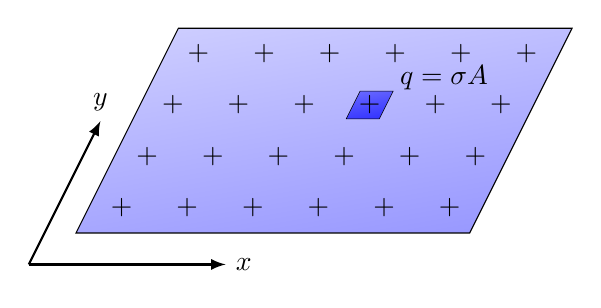
\begin{tikzpicture}[x={(1,0)},y={(0.5,1)}]%,z={(0.73cm,0.73cm)}
  \def\H{2.6}
  \def\W{5.0}
  \def\Nx{6}
  \def\Ny{4}
  \def\h{0.35}
  \def\w{0.42}
  \coordinate (P) at (3.5*\W/\Nx,2.5*\H/\Ny);
  
  % AXES
  \begin{scope}[shift={(-0.08*\W,-0.08*\W)}]
    \draw[->,thick] (0,0) -- (0,0.7*\H) node[above] {$y$};
    \draw[->,thick] (0,0) -- (0.5*\W,0) node[right] {$x$};
  \end{scope}
  
  % PLANE
  \draw[charged]
    (0,0) --++ (\W,0) --++ (0,\H) --++ (-\W,0) -- cycle;
  \foreach \i [evaluate={\x=(\i-0.5)*\W/\Nx;}] in {1,...,\Nx}{
    \foreach \j [evaluate={\y=(\j-0.5)*\H/\Ny;}] in {1,...,\Ny}{
      \node[scale=1.0,rotate=0] at (\x,\y) {$+$};
    }
  }
  
  % CHARGE
  \draw[darkcharged]
    (P) ++ (-\w/2,-\h/2) --++ (\w,0) --++ (0,\h) coordinate (C) --++ (-\w,0) -- cycle;
  \node[above=5,right=-1,scale=1.0] at (C) {$\dd{q}=\sigma \dd{A}$};
  \node[scale=1.0] at (P) {$+$};
  
\end{tikzpicture}
